% \usepackage{adjustbox}
% \usepackage{pifont}
% \usetikzlibrary{babel,quotes,positioning,arrows,snakes,backgrounds,fit,trees,arrows,matrix}

\itemresize{0.8}{$x+y$}

\itemresize{0.8}{a}
\insertequation{x+y}

%\newenvironment{FitToWidth}[1][\linewidth]{%
%	\begin{adjustbox}{width=#1,center}
%	}
%	{\end{adjustbox}}

\clearpage
\createtwocolumn{0.2}{0.2}{7cm}{aaa}{bbbbb}
\createtwocolumn{0.49}{0.49}{0cm}{

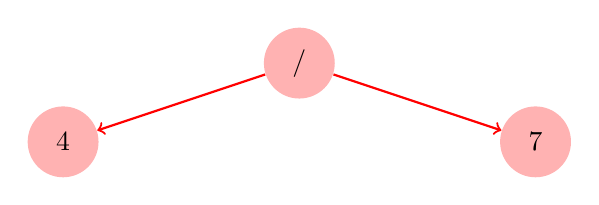
\begin{tikzpicture}[level distance=1.3cm,
level 1/.style={sibling distance=6cm, level distance=1cm},
level 2/.style={sibling distance=3cm, level distance=1cm},
level 3/.style={sibling distance=1.5cm, level distance=1cm}]%Se ocupo para poder separar el arbol creado en una distancia dada
\tikzstyle{every node}=[circle,fill=red!30, inner sep=0pt,minimum size=9mm, node distance=0.5pt]% define el cómo será cada nodo
\tikzstyle{edge from parent}=[red,->,thick,draw] %define el trazado o conexion que abrá entre cada nodo
\node {$/$}%cabeza
child {node {$4$}}
child {node {$7$}%hijo der
};
\end{tikzpicture}

}{

\centering
\begin{tabular}{|ccc|}
	&  & \\ \hline
	& 3 & \\ \hline 
	& x & \\ \hline
	& 2 & \\ \hline
\end{tabular}

}

\begin{adjustbox}{width=\linewidth}
	% \insertequation{a}
	a
\end{adjustbox}
\clearpage
a

\quotes{se desactivaron los quotes <<a>>}

\clearpage

\createhalfcolumnc{
	
	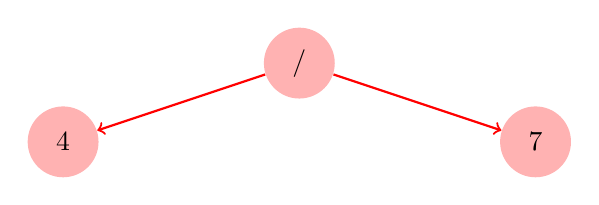
\begin{tikzpicture}[level distance=1.3cm,
	level 1/.style={sibling distance=6cm, level distance=1cm},
	level 2/.style={sibling distance=3cm, level distance=1cm},
	level 3/.style={sibling distance=1.5cm, level distance=1cm}]%Se ocupo para poder separar el arbol creado en una distancia dada
	\tikzstyle{every node}=[circle,fill=red!30, inner sep=0pt,minimum size=9mm, node distance=0.5pt]% define el cómo será cada nodo
	\tikzstyle{edge from parent}=[red,->,thick,draw] %define el trazado o conexion que abrá entre cada nodo
	\node {$/$}%cabeza
	child {node {$4$}}
	child {node {$7$}%hijo der
	};
	\end{tikzpicture}
	
}{
	
	\begin{tabular}{|ccc|}
		&  & \\ \hline
		& 3 & \\ \hline 
		& x & \\ \hline
		& 2 & \\ \hline
	\end{tabular}
	
}